\section[Introduction]{Lecture 1: Introduction}

\subsection{What is Machine Learning?}
Arthur Samuel (1959). Machine Learning: Field of study that gives computers
the ability to learn without being explicitly programmed.
Shapire: Machine learning studies how to automatically learn to make
predictions based on past observations.
The field of machine learning tries to build and understand systems that can
automatically extract information from empirical data in order to improve their
performance.
As a scientific discipline, machine learning is an interdisciplinary (and relatively
young) field focusing both on theoretical foundations of systems that learn,
reason and act as well as on practical applications of these systems.

\textbf{Machine learning draws inspiration and concepts from many scientific fields}

\begin{itemize}
 \item Statistics: Inference from data, probabilistic models, learning theory, ...
 \item Mathematics: Optimization theory, numerical methods, tools for theory, ...
 \item Engineering: Signal processing, system identification, robotics, control, information
theory, data-mining, ...
 \item Computer science: Artificial intelligence, computer vision, information retrieval, datastructures,
implementations ...
 \item Economics: decision theory, operations research, econometrics, ...
 \item Psychology/Cognitive science: Computational linguistics, learning, reinforcement
learning, movement control, ...
 \item Physics: Energy minimization principles, entropy, capacity
 \item Computational Neuroscience: Neural networks, principles of neural information
processing, ...
 \item Frequently: Information flowing back in from application domains, e.g. tools for
bioinformatics getting used in other domains, ...
\end{itemize}

\textbf{Machine learning provides both important statistical tools for
neuroscience as well as a conceptual foundations and inspiration}

\begin{itemize}
\item  Machine learning provides tools for neural data analysis. Examples:
	\begin{itemize}
	\item Use of classification algorithms to decode stimuli/mental representations from
functional imaging data
	\item Methods for spike-sorting
	\item Bayesian inference for psychometric functions
	\item  Predicting spikes from calcium transients
	\item Receptive field mapping
	\item Many, many more...
	\end{itemize}

\item Machine learning provides a conceptual foundation for many tasks in neuroscience
and related fields. How do sensory systems and organisms learn structure from data,
and use this information to make (good or even optimal) decisions? Examples:
	\begin{itemize}
	\item Learning sensory representations from natural stimuli
	\item Bayesian cue-integration
	\item Models of reinforcement learning
	\item Predictive coding
	\item Probabilistic population
	\item Models of memory retrieval
	\item Many, many more...
	\end{itemize}
\end{itemize}

\subsection{The major classes of Machine Learning algorithms}
\textbf{There are three major types of machine learning:
Supervised learning, unsupervised learning and reinforcement learning}\\

Suppose you have some data x1, x2, x3 ...
\begin{itemize}
\item Supervised Learning: You are also given some desired outputs y1, y2, y3, ..., and
your goal is learn a rule/function that you can use to predict yi from xi
\item Unsupervised Learning: Your goal is to build a good model of x that you can use
for decision making, interpretation, other learning tasks, visualization, datacompression,
science, etc...
\item Reinforcement Learning: You have the ability to produce actions a1, a2, a3 ..., and
you will receive rewards (or punishments) r1, r2, r3 ..., depending on your actions, the
state of the environment, as well as your luck. Your goal is to find a strategy that
allows you to maximize your rewards in the long term.
\item Of course, this is a bit of an over-simplification, as there exist many variants of these
types as well as hybrids (semi-supervised learning) and approaches which do not
quite fit into either of the three.
\item We will deal with Supervised Learning (Jakob Macke, Part I) and with Unsupervised
Learning (Matthias Bethge, Part II), but not with Reinforcement Learning
\end{itemize}



\subsection{Introduction to supervised learning}

\textbf{In supervised learning, the machine (or organism) has to predict unknown outputs given some sensory inputs}\\
\begin{itemize}
\item Classification: Predict binary (or categorial) output, e.g:
	\begin{itemize}
    \item Does this example belong to class one or two?
    \item Will a neuron spike in response to this stimulus?
	\item Based on this brain-scan, does this patient have a given disease or not?
	\item Will this customer buy this product or not?
    \end{itemize}

\item Regression: Predict continuous (or multi-valued)output:
	\begin{itemize}
	\item How many spikes will the neuron fire?
    \item How quickly will the disease progress?
	\item How much is this customer willing to pay for this product?
    \end{itemize}

\item Structured output regression: Anything more complex, e.g:
	\begin{itemize}
	\item What patterns of population activity are evoked by some stimulus?
	\item Based on some neural measurement, can you reconstruct the image/movie that was shown?
    \end{itemize}

\end{itemize}

\subsubsection{Polynomial regression}
\begin{figure}
	\centering
	\begin{subfigure}[b]{0.45\textwidth}
                \centering
                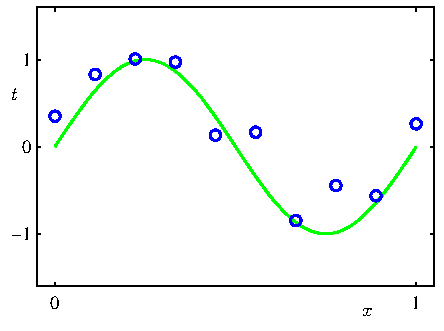
\includegraphics[width=\textwidth]{./lecture1/Figure1_2}
    \end{subfigure}%
	~
	\begin{subfigure}[b]{0.45\textwidth}
                \centering
                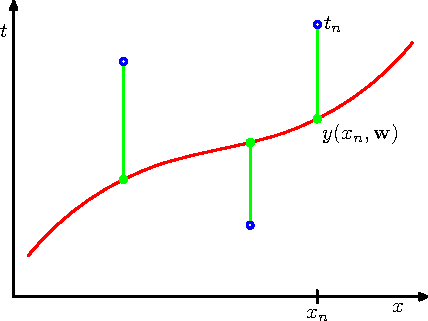
\includegraphics[width=\textwidth]{./lecture1/Figure1_3}
    \end{subfigure}%
	\caption{Figures taken from Bishop.}
\end{figure}

\begin{align*}
	y(x,w) &= w_0 + w_1x + w_2x^2 + . . . + w_Mx^M\\
	E(w) &= \sum_{n=1}^N (y(xn, w) - t_n)^2
\end{align*}

\begin{figure}
	\centering
	\begin{subfigure}[b]{0.45\textwidth}
                \centering
                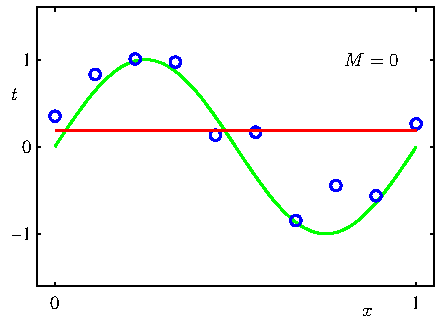
\includegraphics[width=\textwidth]{./lecture1/Figure1_4a}
    \end{subfigure}%
	~
	\begin{subfigure}[b]{0.45\textwidth}
                \centering
                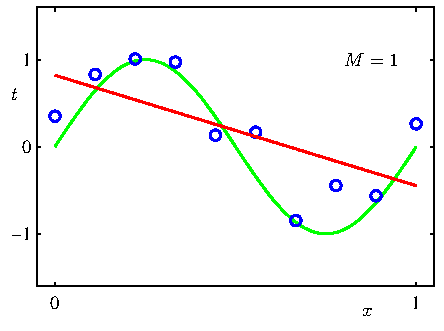
\includegraphics[width=\textwidth]{./lecture1/Figure1_4b}
    \end{subfigure}%
    
    % blank line for new line
    \begin{subfigure}[b]{0.45\textwidth}
                \centering
                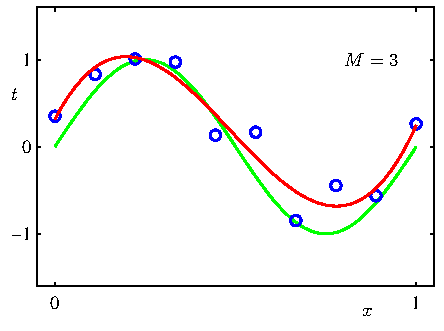
\includegraphics[width=\textwidth]{./lecture1/Figure1_4c}
    \end{subfigure}%
	~
	\begin{subfigure}[b]{0.45\textwidth}
                \centering
                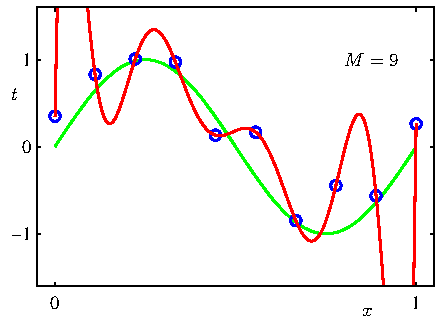
\includegraphics[width=\textwidth]{./lecture1/Figure1_4d}
    \end{subfigure}%
	\caption{Figures taken from Bishop.}
\end{figure}


\subsubsection{Generalization}
\textbf{We are interested in generalization ability. Cross-validation allows you to
quantify how well your algorithm generalizes.}\\
\begin{itemize}
	\item Split your data (randomly) into non-overlapping \textit{training} and \textit{test} sets
    \item Fit parameters on \textit{training set}
    \item Test quality of model by testing how well it fits on the test-set
    \item K-fold cross-validation: Repeat this procedure K times such that every data-point appears exactly once in a test-set.
    \item Cross-validation gives an estimate of the generalization error.
\end{itemize}

\begin{wrapfigure}{r}{0.5\textwidth}
	\centering
	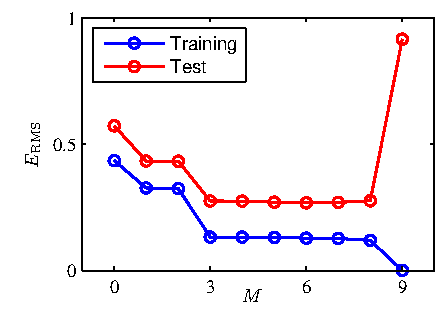
\includegraphics[width=0.45\textwidth]{./lecture1/Figure1_5}
\end{wrapfigure}

\textbf{Regularization protects against over-fitting.}\
\begin{itemize}
 \item Prefer simple explanations (=models) over complex ones: Occams Razor
 \item Trade off between model-complexity and goodness-of-fit
 \item Bayesian approach: Specify a prior distribution over models, and search for a model which both has high probability under the prior AND fits the data well
\end{itemize}

\begin{align*}
	E(w) &= \sum_{n=1}^N (y(x_n, w) - t_n)^2 + \frac{\lambda}{2} \|w\|^2
\end{align*}

\begin{figure}
	\centering
	\begin{subfigure}[b]{0.45\textwidth}
                \centering
                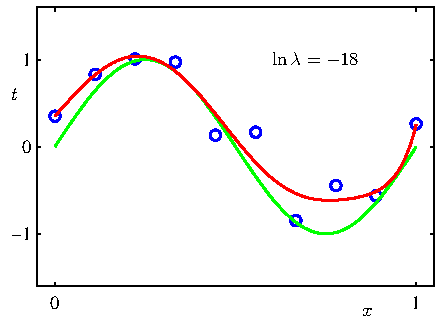
\includegraphics[width=\textwidth]{./lecture1/Figure1_7a}
    \end{subfigure}%
	~
	\begin{subfigure}[b]{0.45\textwidth}
                \centering
                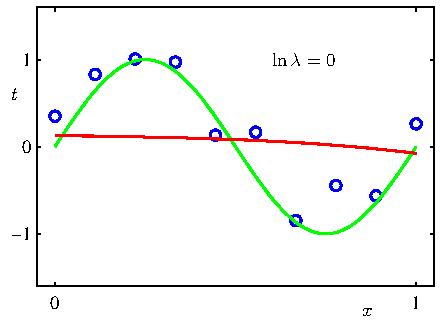
\includegraphics[width=\textwidth]{./lecture1/Figure1_7b}
    \end{subfigure}%
	\caption{Figures taken from Bishop.}
\end{figure}

\subsection{Course objective}
In this course, we follow (and promote) a very statistical (and mostly Bayesian) approach to machine learning
\begin{itemize}
	\item Many approaches in machine learning can be motivated from a statistical perspective.
	\item We will follow a statistical/probabilistic approach, but not be \textit{hard core} Bayesian
	\item Advantages of a probabilistic approach:
	\item Unified theoretical and conceptual framework
	\item Principled methods, e.g. for setting free parameters
	\item Make inferences about missing inputs
	\item Ability to sample from model
	\item Scientific reasoning: Model comparison, hypothesis testing
	\item Connections with neural coding and cognitive models
	\item Disadvantages: mostly computational in nature
	\item Exact solutions are often intractable, and an approximate solution to a great problem can be worse than a simpler approach with an exact solution
	\item \textit{Non Bayesian} algorithms are often faster and more efficient, especially on big data sets.
	\item Famous \textit{non probabilistic} algorithms: e.g. Support Vector Machines, Convolutional Neural Networks
\end{itemize}
